\documentclass[aspectratio=169,11pt]{beamer}

\usepackage[T1]{fontenc}
\usepackage{lmodern}
\usepackage{tikz}
\usepackage{array}
\usepackage{tabularx}
\usepackage{colortbl}
\usetikzlibrary{calc}

\definecolor{paper}{HTML}{FAF7F1}
\definecolor{ink}{HTML}{24283B}
\definecolor{muted}{HTML}{676B78}
\definecolor{coral}{HTML}{D96F55}
\definecolor{amber}{HTML}{D8A640}
\definecolor{blue}{HTML}{607FA5}
\definecolor{violet}{HTML}{8B719C}
\definecolor{rule}{HTML}{DDD7CF}

\setbeamercolor{background canvas}{bg=paper}
\setbeamercolor{normal text}{fg=ink,bg=paper}
\setbeamercolor{frametitle}{fg=ink,bg=paper}
\setbeamerfont{frametitle}{size=\fontsize{30}{34}\selectfont,series=\bfseries}
\setbeamertemplate{navigation symbols}{}
\setbeamertemplate{footline}{}
\setbeamertemplate{itemize item}{\color{coral}\raise0.2ex\hbox{\rule{0.45em}{0.12em}}}
\setbeamertemplate{itemize subitem}{\color{blue}\small\textbullet}
\setlength{\leftmargini}{1.35em}
\setlength{\leftmarginii}{1.25em}

\newcommand{\frametitleline}[1]{%
  \frametitle{#1}\vspace{-0.25em}\textcolor{coral}{\rule{1.05cm}{2pt}}\par\vspace{0.7em}%
}
\newcommand{\quiet}[1]{{\color{muted}#1}}

\title{GutFeeling}
\subtitle{A simple diary for food and digestive symptoms}
\date{}

\begin{document}

% Talk time: about 25 seconds.
\begin{frame}[plain]
  \vspace*{1.05cm}
  {\color{coral}\rule{1.2cm}{3pt}}\par\vspace{0.5cm}
  {\fontsize{46}{52}\selectfont\bfseries GutFeeling\par}
  \vspace{0.55cm}
  {\fontsize{25}{32}\selectfont A simple diary for food and\par digestive symptoms\par}
  \vspace{0.65cm}
  {\fontsize{18}{24}\selectfont\color{muted}
    Helps people notice possible patterns over time.\par}
  \vfill
  {\small\color{muted}Project idea\hspace{0.35cm}/\hspace{0.35cm}3--5 minute pitch}
  \vspace{0.45cm}
\end{frame}

% Talk time: about 40 seconds.
\begin{frame}
  \frametitleline{Why a food diary can help}
  \vspace{0.15cm}
  {\fontsize{23}{31}\selectfont
    Meals are easy to forget.\par\vspace{0.38cm}
    Symptoms may begin hours later.\par\vspace{0.38cm}
    Stress and daily routines can also affect how someone feels.\par}
  \vfill
  
\begin{tikzpicture}[x=1cm,y=1cm]
    \draw[rule,line width=1.2pt] (0,0) -- (11.8,0);
    \foreach \x/\c in {0.25/coral,3.9/amber,7.75/blue,11.35/violet}{
      \fill[\c] (\x,0) circle (0.10);
    }
    \node[anchor=north west,align=left,text width=2.7cm,font=\small\color{muted}] at (0.05,-0.18) {Meal};
    \node[anchor=north west,align=left,text width=2.7cm,font=\small\color{muted}] at (3.7,-0.18) {Later that day};
    \node[anchor=north west,align=left,text width=2.7cm,font=\small\color{muted}] at (7.55,-0.18) {Symptom note};
    \node[anchor=north west,align=left,text width=2.7cm,font=\small\color{muted}] at (11.15,-0.18) {Next day};
  \end{tikzpicture}
  \vspace{0.55cm}
  {\large\bfseries GutFeeling keeps these notes together across days.}
\end{frame}

% Talk time: about 60 seconds.
\begin{frame}
  \frametitleline{A diary in three quick steps}
  \vspace{0.25cm}
  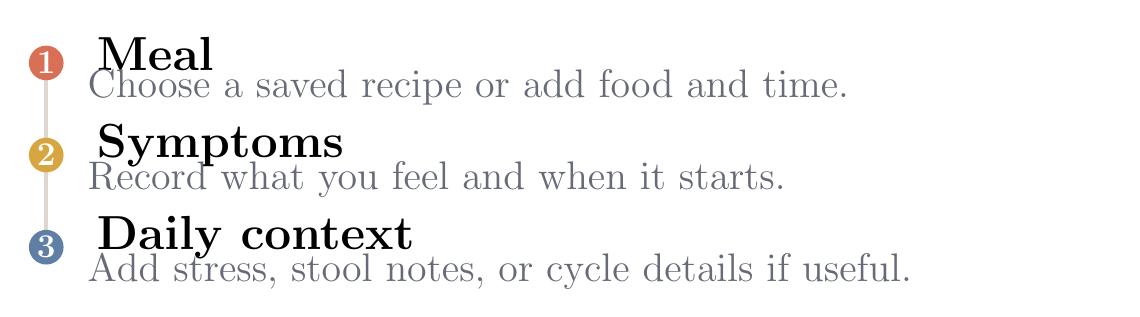
\begin{tikzpicture}[x=1cm,y=1cm]
    \draw[rule,line width=1.5pt] (0.38,0) -- (0.38,-2.34);
    \foreach \y/\c/\n in {0/coral/1,-1.17/amber/2,-2.34/blue/3}{
      \fill[\c] (0.38,\y) circle (0.22);
      \node[font=\bfseries\large,text=white] at (0.38,\y) {\n};
    }
    \node[anchor=west,font=\bfseries\fontsize{19}{23}\selectfont] at (0.9,0.12) {Meal};
    \node[anchor=west,align=left,text width=13cm,inner sep=0pt,font=\fontsize{15}{18}\selectfont,text=muted] at (0.9,-0.31) {Choose a saved recipe or add food and time.};
    \node[anchor=west,font=\bfseries\fontsize{19}{23}\selectfont] at (0.9,-1.05) {Symptoms};
    \node[anchor=west,align=left,text width=13cm,inner sep=0pt,font=\fontsize{15}{18}\selectfont,text=muted] at (0.9,-1.48) {Record what you feel and when it starts.};
    \node[anchor=west,font=\bfseries\fontsize{19}{23}\selectfont] at (0.9,-2.22) {Daily context};
    \node[anchor=west,align=left,text width=13cm,inner sep=0pt,font=\fontsize{15}{18}\selectfont,text=muted] at (0.9,-2.65) {Add stress, stool notes, or cycle details if useful.};
  \end{tikzpicture}
  \vfill
  {\fontsize{16}{19}\selectfont Recipes can be imported from a web link, then checked and edited.}
\end{frame}

% Talk time: about 65 seconds.
\begin{frame}
  \frametitleline{The app looks for repeated patterns}
  \begin{columns}[T,onlytextwidth]
    \begin{column}{0.56\textwidth}
      {\fontsize{21}{28}\selectfont
        It compares meals, ingredients and symptom timing across days.\par\vspace{0.45cm}
        It includes context such as stress and optional cycle notes.\par\vspace{0.45cm}
        Users can flag a recipe they suspect and correct diary entries later.\par}
    \end{column}
    \begin{column}{0.38\textwidth}
      \vspace{0.12cm}
      {\color{coral}\rule{0.08cm}{3.3cm}}\hspace{0.28cm}%
      \begin{minipage}[t]{0.88\linewidth}
        {\large\bfseries What the user gets}\par\vspace{0.2cm}
        {\large\color{muted}
          Possible food links to review\par\vspace{0.28cm}
          A view of other factors\par\vspace{0.28cm}
          A short report to share with a health professional}
      \end{minipage}
    \end{column}
  \end{columns}
  \vfill
  \textbf{The app shows possible links, not a medical diagnosis.}
\end{frame}

% Talk time: about 55 seconds.
\begin{frame}
  \frametitleline{An eight-week project plan}
  {\large Four two-week sprints, managed in Linear and Tiny Scrum.}\par
  \vspace{0.5cm}
  \begin{center}
  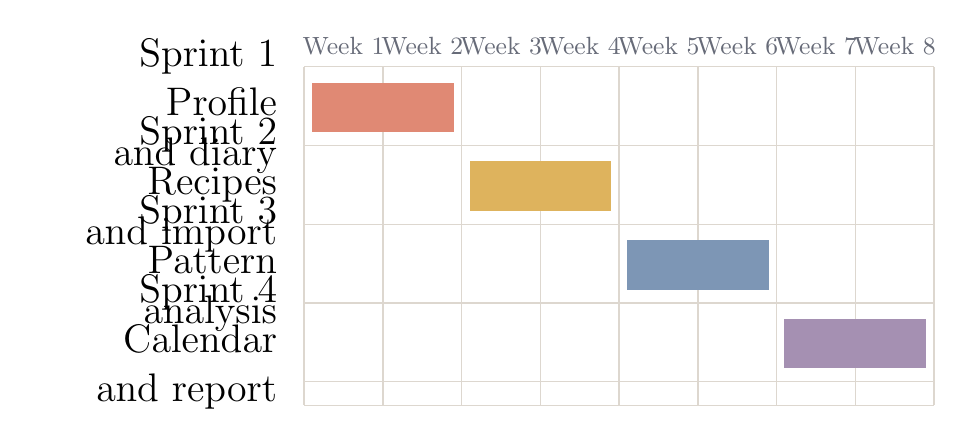
\begin{tikzpicture}[x=1.0cm,y=1cm]
    % Week grid. Each shaded bar covers two weeks, or one sprint.
    \foreach \x/\week in {0/1,1/2,2/3,3/4,4/5,5/6,6/7,7/8}{
      \node[font=\small\color{muted}] at (\x+0.5,0.32) {Week \week};
      \draw[rule,line width=0.5pt] (\x,0.05) -- (\x,-4.25);
    }
    \draw[rule,line width=0.5pt] (8,0.05) -- (8,-4.25);
    \foreach \y in {0.05,-0.95,-1.95,-2.95,-3.95,-4.25}{
      \draw[rule,line width=0.5pt] (0,\y) -- (8,\y);
    }
    \node[anchor=east,align=right,text width=3.05cm,font=\fontsize{15}{18}\selectfont] at (-0.22,-0.45) {Sprint 1\\Profile and diary};
    \node[anchor=east,align=right,text width=3.05cm,font=\fontsize{15}{18}\selectfont] at (-0.22,-1.45) {Sprint 2\\Recipes and import};
    \node[anchor=east,align=right,text width=3.05cm,font=\fontsize{15}{18}\selectfont] at (-0.22,-2.45) {Sprint 3\\Pattern analysis};
    \node[anchor=east,align=right,text width=3.05cm,font=\fontsize{15}{18}\selectfont] at (-0.22,-3.45) {Sprint 4\\Calendar and report};
    \fill[coral!82] (0.10,-0.78) rectangle (1.90,-0.15);
    \fill[amber!85] (2.10,-1.78) rectangle (3.90,-1.15);
    \fill[blue!82] (4.10,-2.78) rectangle (5.90,-2.15);
    \fill[violet!78] (6.10,-3.78) rectangle (7.90,-3.15);
  \end{tikzpicture}
  \end{center}
  \vspace{-0.12cm}
  \begin{center}
    {\large Each sprint ends with a review and retrospective.}
  \end{center}
  \vfill
  {\small\color{muted}The weeks are relative to the project start.}
\end{frame}

\end{document}
